% -*- latex -*-
%%%%%%%%%%%%%%%%%%%%%%%%%%%%%%%%%%%%%%%%%%%%%%%%%%%%%%%%%%%%%%%%
%%%%%%%%%%%%%%%%%%%%%%%%%%%%%%%%%%%%%%%%%%%%%%%%%%%%%%%%%%%%%%%%
%%%%
%%%% This text file is part of the source of slides for
%%%% `Introduction to High-Performance Scientific Computing'
%%%% by Victor Eijkhout, copyright 2012-2020
%%%%
%%%%%%%%%%%%%%%%%%%%%%%%%%%%%%%%%%%%%%%%%%%%%%%%%%%%%%%%%%%%%%%%
%%%%%%%%%%%%%%%%%%%%%%%%%%%%%%%%%%%%%%%%%%%%%%%%%%%%%%%%%%%%%%%%

\Level 1 {Computational aspects of iterative methods}

\begin{frame}{What's in an iterative method?}
  From easy to hard
  \begin{itemize}
  \item Vector updates\\
    These are trivial
  \item Inner product
  \item Matrix-vector product
  \item Preconditioner solve
  \end{itemize}
\end{frame}

\begin{frame}{Inner products: collectives}
  Collective operation: data from all processes is combined.\\
  (Is a matrix-vector product a collective?)

  Examples: sum-reduction, broadcast\\
  These are each other's mirror image, computationally.
\end{frame}

\begin{frame}{Naive realization of collectives}
  Broadcast:
  
  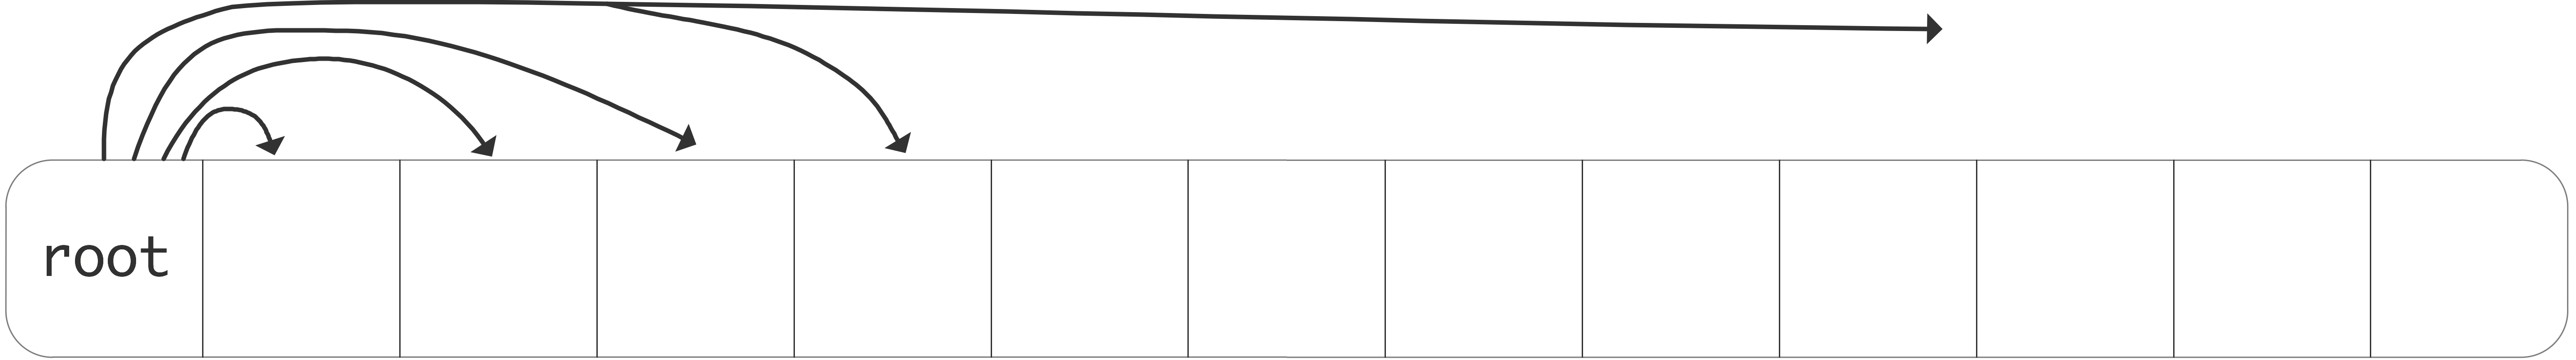
\includegraphics[scale=.06]{bcast-simple}

  Single message:
  \[ \alpha=\hbox{message startup}\approx 10^{-6}s,\qquad
  \beta=\hbox{time per word}\approx 10^{-9}s
  \]
  \begin{itemize}
  \item<1-> Time for message of $n$ words: \[ \alpha +\beta n \]
  \item<2-> Single inner product: $n=1$
  \item<3-> Time for collective?
  \item<4-> Can you improve on that?
  \end{itemize}

\end{frame}

\begin{frame}{Better implementation of collectives}
  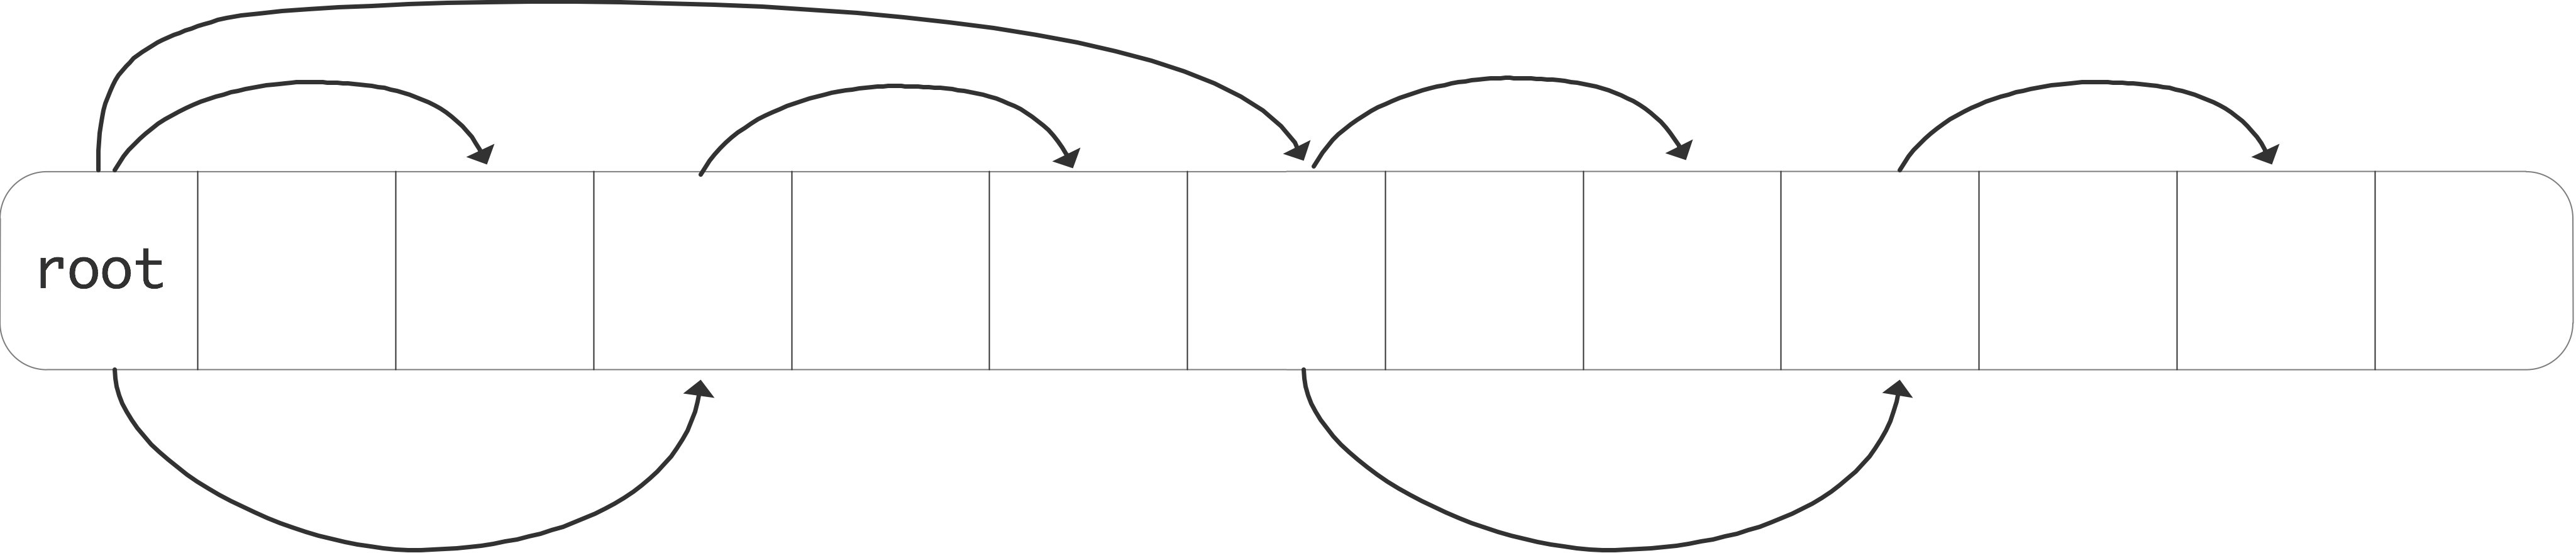
\includegraphics[scale=.07]{bcast-tree}
  
  \begin{itemize}
  \item<1->
    What is the running time now?
  \item<2->
    Can you come up with lower bounds on the $\alpha,\beta$ terms? Are
    these achieved here?
  \item<3-> How about the case of really long buffers?
  \end{itemize}

\end{frame}

\begin{frame}{Inner products}
  \begin{itemize}
  \item Only operation that intrinsically has a $p$ dependence
  \item Collective, so induces synchronization
  \item $\Rightarrow$ exposes load unbalance, can take lots of time
  \item Research in approaches to hiding: overlapping with other operations
  \end{itemize}
\end{frame}

\begin{frame}{What do those inner products serve?}
  \begin{itemize}
  \item Orthogonality of residuals
  \item Basic algorithm: Gram-Schmidt
  \item one step: given $u,v$
    \[ v'\leftarrow v-\frac{u^tv}{u^tu}u. \]
    then $v'\perp u$
  \item bunch of steps: given $U,v$
    \[ v'\leftarrow v-\frac{U^tv}{U^tU}U. \]
    then $v'\perp U$.
  \end{itemize}
  Gram-Schmidt algorithm
\end{frame}

\begin{frame}{Modified Gram-Schmidt}
    \begin{tabbing}
    For \=$i=1,\ldots,n$:\\
    \>let $c_i=u_i^tv/u_i^tu_i$\\
    \>update $v\leftarrow v-c_iu_i$
  \end{tabbing}

    More numerical stable
\end{frame}

\frame{\frametitle{Full Orthogonalization Method}

\begin{quote}
  \begin{tabbing}
    Let $r_0$ be given\\
    For \=$i\geq 0$:\\
    \>let $s\leftarrow K\inv r_i$\\
    \>let $t\leftarrow AK\inv r_i$\\
    \>for \=$j\leq i$:\\
    \>\>let $\gamma_j$ be the coefficient so that $t-\gamma_jr_j\perp r_j$\\
    \>for \=$j\leq i$:\\
    \>\>form \=$s\leftarrow s-\gamma_jx_j$\\
    \>\>and  \>$t\leftarrow t-\gamma_jr_j$\\
    \>let $x_{i+1}=(\sum_j\gamma_j)\inv s$,
    $r_{i+1}=(\sum_j\gamma_j)\inv t$.\\
  \end{tabbing}
\end{quote}
}

\frame{\frametitle{Modified Gramm-Schmidt}
\begin{quote}
  \begin{tabbing}
    Let $r_0$ be given\\
    For \=$i\geq 0$:\\
    \>let $s\leftarrow K\inv r_i$\\
    \>let $t\leftarrow AK\inv r_i$\\
    \>for \=$j\leq i$:\\
    \>\>let $\gamma_j$ be the coefficient so that $t-\gamma_jr_j\perp r_j$\\
    \>\>form \=$s\leftarrow s-\gamma_jx_j$\\
    \>\>and  \>$t\leftarrow t-\gamma_jr_j$\\
    \>let $x_{i+1}=(\sum_j\gamma_j)\inv s$,
    $r_{i+1}=(\sum_j\gamma_j)\inv t$.\\
  \end{tabbing}
\end{quote}
}

\frame{\frametitle{Practical differences}
  \begin{itemize}
  \item Modfied GS more stable
  \item Inner products are global operations: costly
  \end{itemize}
}

\begin{comment}
  \begin{frame}{Block methods}
    \begin{itemize}
    \item GMRES does a block orthogonalization in every iteration
    \item in Conjugate Gradients:
      \begin{itemize}
      \item single orthogonalization
      \item matrix-vector product
      \end{itemize}
      (this is actually kinda modified Gram-Schmidt)
    \item $\Rightarrow$ communication minimization through block methods:\\
      compute $x,Ax,A^2x,\ldots,A^kx$, then block orthogonalize
    \item latency hiding vs numerical stability
    \end{itemize}
  \end{frame}
\end{comment}

\Level 2 {Matrix-vector product}

\begin{frame}{PDE, 2D case}
    A difference stencil applied to a two-dimensional square
    domain, distributed over processors. Each point connects to
    neighbours $\Rightarrow$ each process connects to neighbours.

    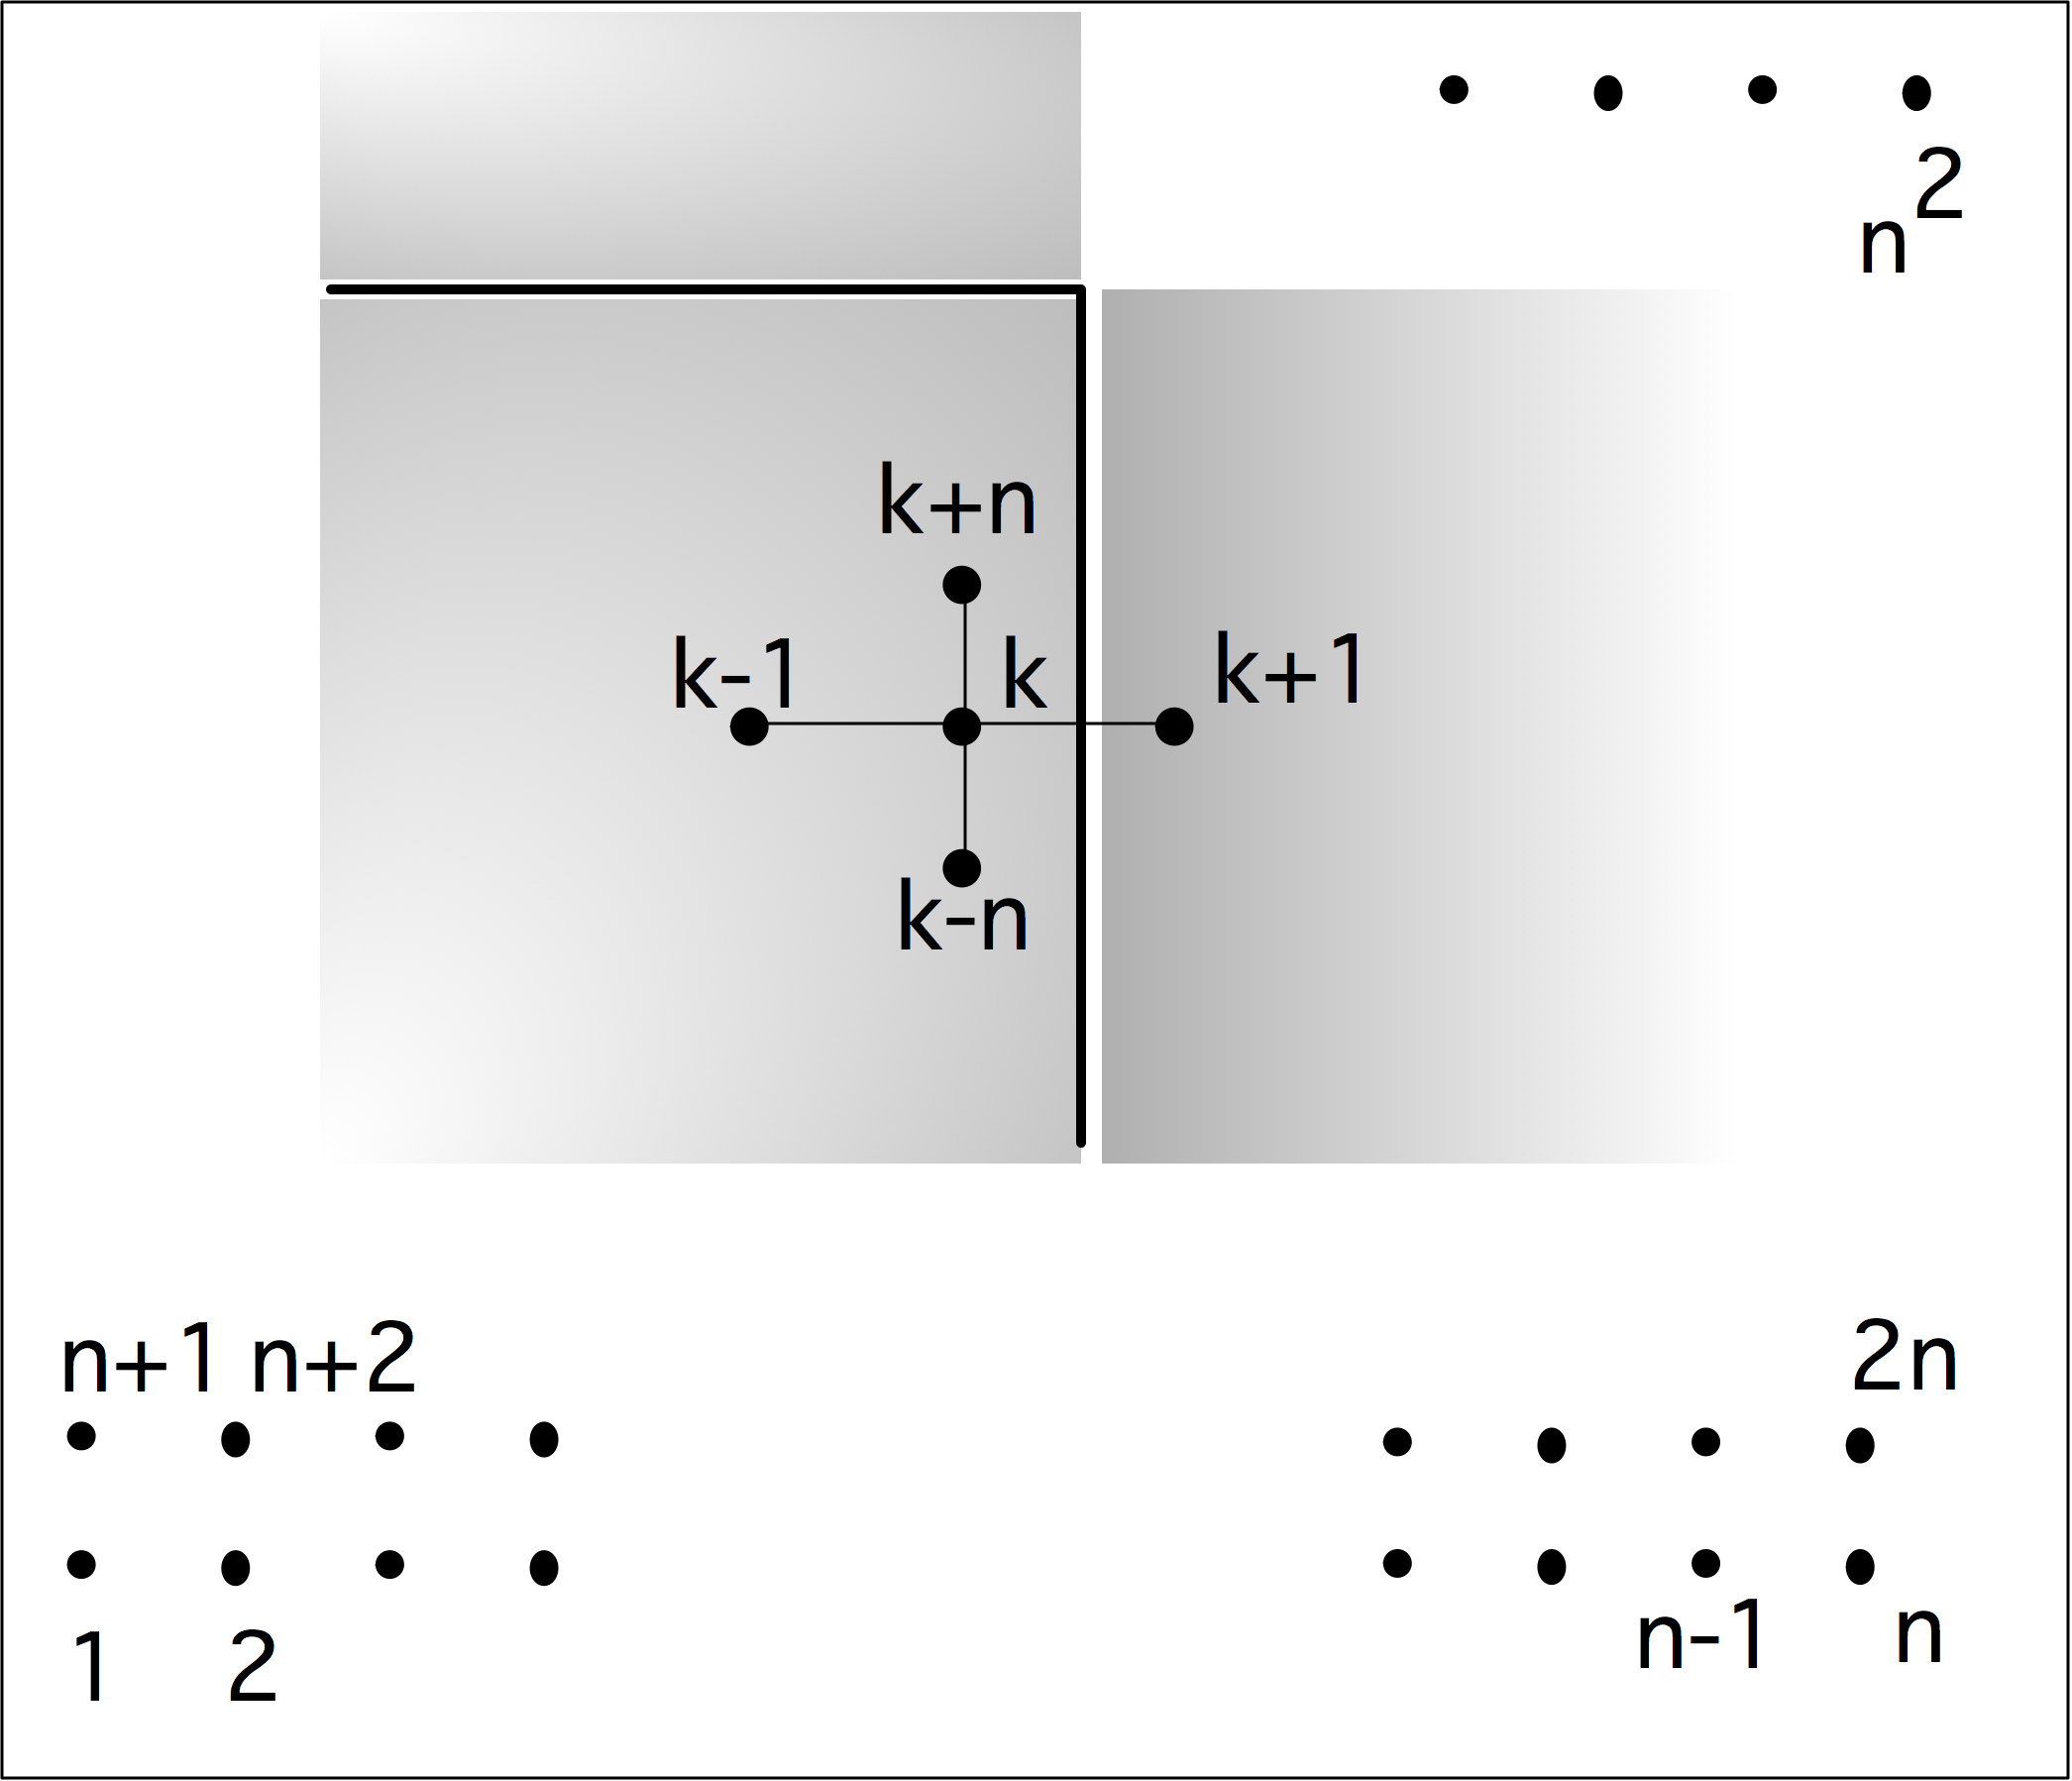
\includegraphics[scale=.1]{laplaceparallel}
\end{frame}

\begin{frame}{Parallelization}
  Assume each process has the matrix values and vector values in part
  of the domain.

  
\includegraphics[scale=.3]{pmvp-1d}

  \onslide<2->{Processor needs to get values from neighbors.}
  
\end{frame}

\begin{frame}{Halo region}
  The `halo' region of a process, induced by a stencil

  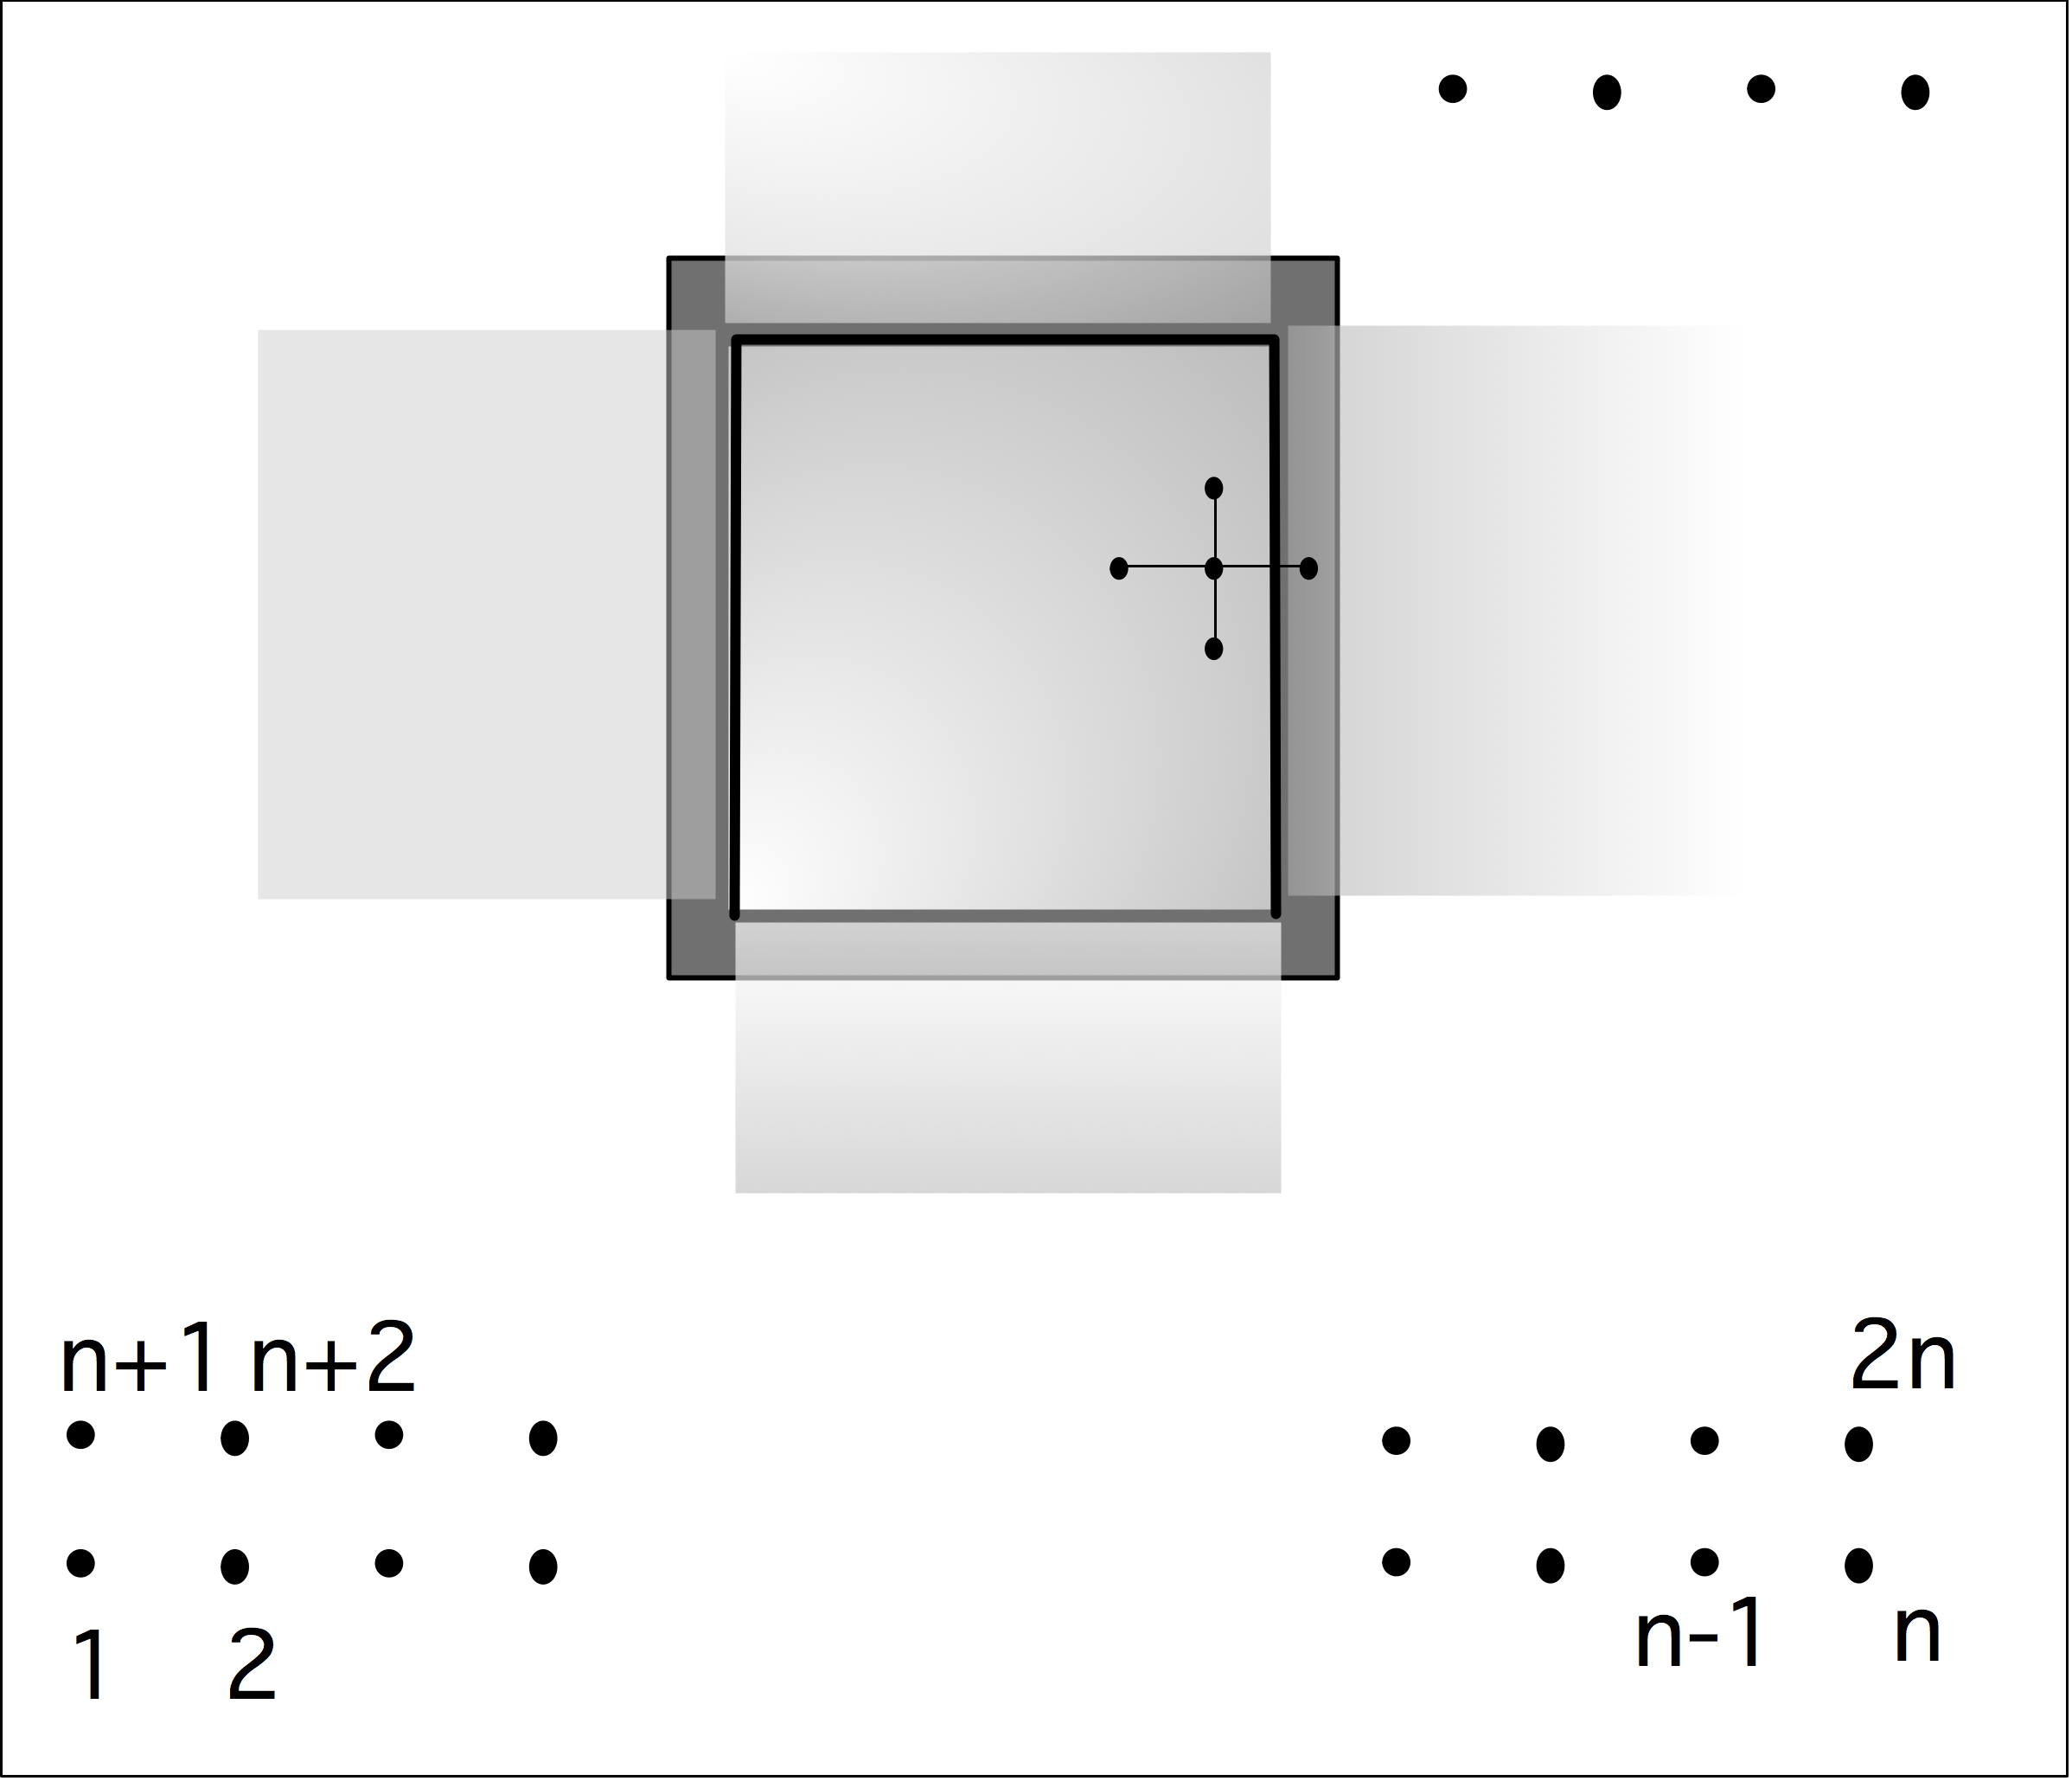
\includegraphics[scale=.1]{laplaceghost}
\end{frame}

\begin{frame}{Matrices in parallel}
  \[ y\leftarrow Ax\]
  and $A,x,y$ all distributed:

  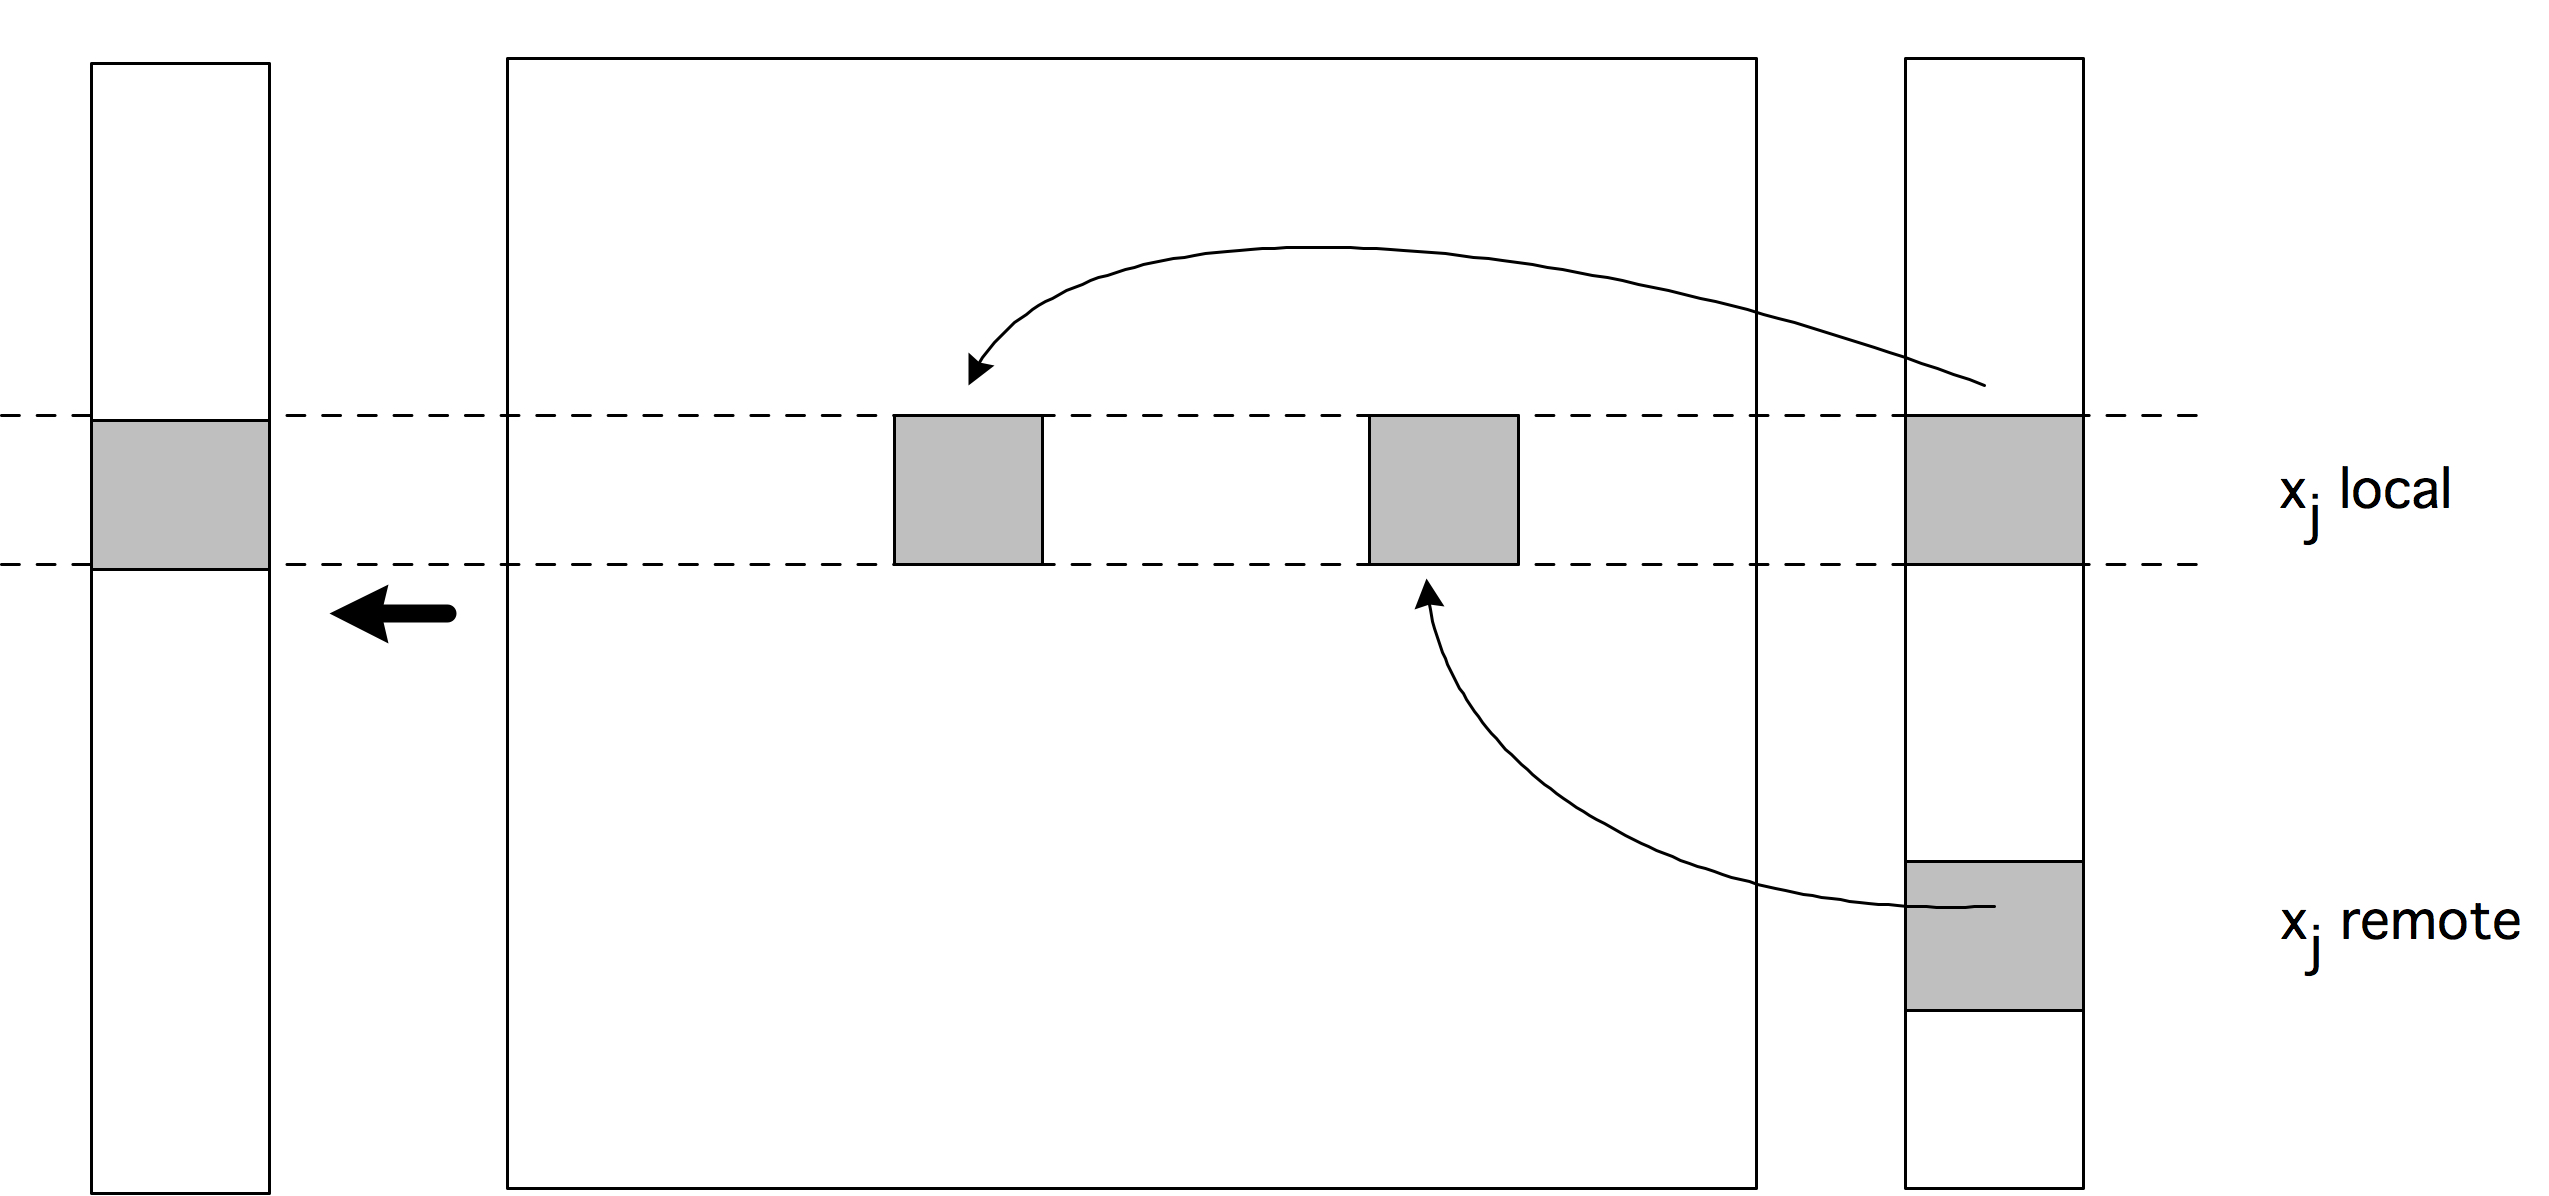
\includegraphics[scale=.12]{distmvp}
\end{frame}

\begin{frame}{Matrix-vector product performance}
  \begin{itemize}
  \item Large scale:
    \begin{itemize}
    \item partition for scalability
    \item minimize communication (Metis, Zoltan: minimize edge cuts)
    \item dynamic load balancing? requires careful design
    \end{itemize}
  \item Processor scale: 
    \begin{itemize}
    \item Performance largely bounded by bandwidth
    \item Some optimization possible
    \end{itemize}
  \end{itemize}
  Beware of optimizations that change the math!
\end{frame}

\Level 2 {Preconditioners}

\begin{frame}{Preconditioners}
  \begin{itemize}
  \item There's much that can be said here.
  \item Some comments to follow
  \item There is intrinsic dependence in solvers, hence in preconditioners:\\
    parallelism is very tricky.\\
    approximate inverses
  \end{itemize}
\end{frame}

